\graphicspath{{detail_design/fig/}}

\chapter{Detail Designs}
\label{chap:detail_design}

\section{Micro-controller}
% discuss how all functional blocks connect and communicate with each other 
The Adafruit STM32F405 feather has a supply voltage of 3.7V and consumes up to $80mA$ when operational, it is powered by a 5000mAh 3.7V lithium polymer 
battery connected with a jst connection. The board features a 3.3V regulator which is to regulate the battery power, there are also pins to distribute 
the 3.3V regulated power off-board. The 3.3V regulator is used to power the GPS receiver, MPU-9250/6500 IMU, and the micro-SD socket. The board has a USB-C 
female connector which is used to load the main program and for debugging during the design process. The board is capable of running circuit python, which was
used in the development of this project. 
%Not sure if i should mention this :(


\section{GPS receiver}
The GPS receiver has a power supply voltage of 3.3V and is powered by the Feathers 3.3V regulator. It is connected to a pin on the feather which is 
configured as UART, with a BAUD rate of 9600. The GPS receiver continually receives data at a frequency which is set during the configuration process, in 
this case its every second. Data sent by the GPS receiver is in the form of ASCII encoded sentences which follow the NMEA protocol\cite{nmea}. The NMEA 
protocol defines a number of ASCII identifiers which occur at the beginning of each ASCII sentence, they are used to identify the type of data 
contained in the sentence. Table \ref{table:NMEA} shows the specific NMEA sentences which are relevant to this project and their corresponding ASCII 
identifiers.
\\

\begin{table}[!h]
    \centering
    \caption{NMEA sentence information}
    \label{table:NMEA}
    \begin{tabular}{ | m{10em} | m{25em} | }
        
        \hline
        \textbf{Sentence identifier} & \textbf{Description} \\
        \hline
        \$GPGGA & Global Positioning System Fix Data (Time, Latitude, Longitude) \\
        \hline
        \$GPGLL & Geographic Position, Latitude / Longitude and time. \\
        \hline
        \$GPGSV & GPS Satellites in view \\
        \hline
        \$GPVTG & Track Made Good and Ground Speed. \\
        \hline
        \$GPRMC & Recommended minimum specific GPS/Transit data (Latitude, Longitude, Speed over ground in knots, Track angle made true, Magnetic variation) \\
        \hline
    \end{tabular}
\end{table}

% Not sure it uses PMTK
% The GPS receiver can be configured by sending the appropriate PMTK command packets\cite{pmtk}. These commands are the same for all GPS receivers. The GPS receiver was
% set to send GGA and RMC NMEA sentences, and the update rate was set to $2Hz$ by sending the appropriate PMTK commands.

\section{Wind Direction Sensor}
The wind direction sensor has a supply voltage in the range 12~30VDC, and is powered by two 9V alkaline batteries in series. It is mounted on the bow of the vessel.
It outputs a $4-20mA$ analog signal,
which is connected directly to pin A4 of the Feather. Pin A4 on the Feather connects to a 5V tolerant pin on the STM32F405 micro-controller. This pin was 
configured to use one of the micro-controllers 12-bit ADC, which has a sampling range of $0V$ to $3.3V$. A shunt resistor with a value of $160\Omega$ is 
connected to the sensor output. This value was calculated to produce a voltage over the resister in the range of $642mV$ to $3.2V$. The Actual voltage range
measured over the shunt resister was $642mV$ to $3.07V$.

All pins on the STM32F405 micro-controller are capable of sinking or sourcing $25mA$ maximum, there is therefore no chance of the sensor damaging the micro-controller
pin. A digital buffer was initially considered to prevent the micro-controller from loading the sensor output circuit, but was not used as the ADC inputs are
high impedance. The STM32F405 data sheet\cite{STM32F405-datasheet} specifies that for an ADC input, the max external impedance allowed for an error below $1/4$ of the LSB is $50K\Omega$. 
The shunt resistors value is multitudes smaller than this.     

\section{Servo Motors}
Both the rudder servo motor and the sail servo winch are powered by a 6V source consisting of four 1.5V alkaline batteries. The rudder servo motor is connected to pin
A2 of the feather, the Sail winch servo motor is connected to pin D9 of the Feather. Both these pins are configured to output a 50HZ PWM signal, with a duty cycle set
by the rudder and sail position controllers. The rudder angle is measured from the centre line of the boat, this corresponds to the neutral position of the rudder. Positive 
rudder angle is measured from neutral position to the starboard side of the vessel, negative rudder angle is measured from the neutral position to port side of the vessel. 
Sail position is measured in degrees from the centre line of the vessel to either the port or starboard side. The maximum and minimum PWM values for both servo motors was 
determined experimentally and is summarized in table \ref{table:pwm}, along with the corresponding angles. Note that the sail position minimum angle is $10^{\circ}$, this 
is in accordance with the recommendations outlined in the sailboats manual.

\begin{table}[!h]
    \centering
    \caption{Servo motor PWM limits}
    \label{table:pwm}
    \begin{tabularx}{\columnwidth}{ | X | X | X | X | X | }
        
        \hline
        Servo motor & PWM\_Min & PWM\_Min corresponding angle & PWM\_Max & PWM\_Max corresponding angle \\
        \hline
        Rudder & 48 & $60^{\circ}$ & 102 & $-60^{\circ}$ \\
        \hline
        Sail & 75 &  $10^{\circ}$ & 120 & $80^{\circ}$ \\
        \hline
    \end{tabularx}
\end{table}

\section{Micro-SD card}
The micro-SD card socket has a supply voltage of 3.3V and is powered with the Feathers 3.3V regulator. It is connected to the Feather using a SPI interface. The micro-SD card sockets MOSI, MISO,
 and clock lines are connected directly to the corresponding pins on the Feather, the chip select line is connected to pin 6 of the Feather. The micro-SD card is formatted with the FAT32 file 
 system, and as, such writing to the micro-SD card is done with FAT32 protocol.


\section{Digital compass}
The MPU-9250/6500 IMUhas a supply voltage of 3.3V and is powered by the Feather boards 3.3V regulator. It is connected to the Feather via a $I^{2}C$ connection. The IMU has an address pin 
which is grounded. The purpose of the address pin is for setting the LSB of the $I^{2}C$, this allows two IMU's to be connected to the same bus, which is not needed in this case. 

\subsection{Tilt Compensation}

To perform tilt compensation, firstly pitch and roll angles of the inertial frame of the vessel must be found. Eq. \ref{eq:acc_1} is used to transform a sampled acceleration vector back to 
the NED frame of reference, where there exists only a z-component with magnitude 9.81 $m/s^2$. In this eqution $\vec{A}_s$ represents the acceleration vector which has been 
sampled from the IMU, g is acceleration due to gravity and $\vec{R_{x,\phi}}$, $\vec{R_{y,\theta}}$, $\vec{R_{z,\psi}}$ represent equations \ref{eq:R_x}, \ref{eq:R_y}, \ref{eq:R_z} 
respectively. 

\begin{equation}
    \label{eq:acc_1}
    \vec{R_{y,\theta}} \cdot \vec{R_{x,\phi}} \cdot \vec{A_s} = \begin{bmatrix} 0 & 0 & g \end{bmatrix}^T
\end{equation}

Expanding Eq. \ref{eq:acc_1}, gives Eq. \ref{eq:acc_1_expand}. The components of the sampled acceleration vector are $A_{sx}$, $A_{sy}$ and $A_{sz}$.

\begin{equation}
    \label{eq:acc_2}
    \begin{bmatrix} cos\theta & 0 & sin\theta \\ 0 & 1 & 0 \\ -sin\theta & 0 & cos\theta \end{bmatrix} \begin{bmatrix} 1 & 0 & 0 \\ 0 & cos\phi & -sin\phi \\ 0 & sin\phi & cos\phi \end{bmatrix} \begin{bmatrix} A_{sx} \\ A_{sy} \\ A_{sz} \end{bmatrix}= \begin{bmatrix} 0 \\ 0 \\ g \end{bmatrix}
\end{equation}

Expanding Eq.\ref{eq:acc_2} further gives Eq.\ref{eq:acc_3},then Eq. \ref{eq:acc_4} and \ref{eq:acc_5}.

\begin{equation}
    \label{eq:acc_3}
    \begin{bmatrix} cos\theta & sin\theta sin\phi & sin\theta cos\phi \\ 0 & cos\phi & -sin\phi \\ -sin\theta & cos\theta sin\phi & cos\theta cos\phi \end{bmatrix} \begin{bmatrix} A_{sx} \\ A_{sy} \\ A_{sz} \end{bmatrix}= \begin{bmatrix} 0 \\ 0 \\ g \end{bmatrix}
\end{equation}

\begin{equation}
    \label{eq:acc_4}
    A_{s,x}cos\theta + A_{s,y}sin\theta sin\phi + A_{s,z}sin\theta cos\phi = 0
\end{equation}

\begin{equation}
    \label{eq:acc_5}
    A_{s,y}cos\phi - A_{s,z}sin\phi = 0
\end{equation}

Roll angle $\phi$ can be found using Eq.\ref{eq:roll} which results from rearranging terms in Eq.\ref{eq:acc_5}

\begin{equation}
    \label{eq:roll}
    \phi = \arctan \left(\frac{A_{s,y}}{A_{s,z}}\right)
\end{equation}

By substituting roll angle $\phi$ into Eq.\ref{eq:pitch} - which is derived from Eq.\ref{eq:acc_4} - pitch angle $\theta$ is found.

\begin{equation}
    \label{eq:pitch}
    \theta = \arctan \left( \frac{ -A_{s,x}}{A_{s,y}sin\phi + A_{s,z}cos\phi}\right)
\end{equation}

Now that pitch and roll angles of the inertial frame of the vessel are known, a sampled magnetometer vector - $\vec{B_{s}}$ - can be transformed to the NED frame of reference. This is done
using Eq.\ref{eq:mag_1}, where $\vec{B_{r}}$ is the transformed vector. Eq.\ref{eq:R_z} is not used here as this will eliminate yaw angle $\psi$ whixh in needed to determine the resulting bearing

\begin{equation}
    \label{eq:mag_1}
    \vec{B_{r}} = \vec{R_{y,\theta}} \cdot \vec{R_{x,\phi}} \cdot \vec{B_{s}}
\end{equation}

Eq.\ref{eq:mag_1} is then expanded, giving Eq.\ref{eq:mag_2} and Eq.\ref{eq:mag_3}.

\begin{equation}
    \label{eq:mag_2}
    \begin{bmatrix} B_{r,x} \\ B_{r,y} \\ B_{r,z} \end{bmatrix} = \begin{bmatrix} cos\theta & 0 & sin\theta \\ 0 & 1 & 0 \\ -sin\theta & 0 & cos\theta \end{bmatrix} \begin{bmatrix} 1 & 0 & 0 \\ 0 & cos\phi & -sin\phi \\ 0 & sin\phi & cos\phi \end{bmatrix} \begin{bmatrix} B_{s,x} \\ B_{s,y} \\ B_{s,z} \end{bmatrix}
\end{equation}

\begin{equation}
    \label{eq:mag_3}
    \begin{bmatrix} B_{r,x} \\ B_{r,y} \\ B_{r,z} \end{bmatrix} = \begin{bmatrix} B_{s,x} cos\theta + B_{s,y} sin\theta sin\phi + B_{s,z} sin\theta cos\phi \\ 0 + B_{s,y} cos\phi - B_{s,z} sin\phi \\ -B_{s,x} sin\theta +  B_{s,y} cos\theta sin\phi + B_{s,z} cos\theta cos\phi \end{bmatrix} 
\end{equation}
\\

Eq.\ref{eq:yaw} is now derived using Eq.\ref{eq:mag_3}, where yaw angle $\psi$ represents the tilt compensated heading of the vessel. The ATAN2() function in python is used to determine 
the yaw angle, it returns a value in the range of $-180^{\circ}$ to $180^{\circ}$. The following check is therefore done in software: if the yaw angle is negative then $360^{\circ}$ is added
to it. This ensures bearing is in the range $0^{\circ}$ to $360^{\circ}$.

\begin{equation}
    \label{eq:yaw}
    \psi =  \left(\frac{-B_{r,y}}{B_{r,x}}\right) \newline
        =\arctan \left(\frac{B_{s,z} sin\phi - B_{s,y} cos\phi }  {B_{s,x} cos\theta + B_{s,y} sin\theta sin\phi + B_{s,z} sin\theta cos\phi}\right)
\end{equation}

\subsection{Calibration}
As mentioned in sec.\ref{}, the earths magnetic field varies in strength and orientation depending on location, ferrous metals nearby the digital compass can also distort the local magnetic field
(this could be interference from other compenents), the digital compass therefore needs to be calibrated to compensate for this. Two disturbances in the 
earths magnetic field are compensated for during a calibration process, they include: hard-iron effects and soft-iron disturbances. Hard-iron effects adds a constant magnitude field component along
each axis of the sampled magnetic field values. Soft-iron disturbances arise from interaction of the earths magnetic field, the amount of distortion varies depending on the orientation of the digital 
compass. 

The calibration process is done by rotating the digital compass in such a manner that every axis aligns with all other axes at least once, while this is done, samples from the magnetometer 
are taken. The maximum and minimum values found along each axis during this process are stored. Eq.\ref{eq:hard-iron} and Eq.\ref{eq:soft-iron_3} are used to determine hard-iron offsets 
and soft iron values for each axis respectively. After the calibration process has concluded, hard-iron offset is subtracted and soft-iron corection is applied to every sampled value. Eq.\ref{eq:calibrate}
shows how this is done.

\begin{equation}
    \label{eq:hard-iron}
    \begin{bmatrix} offset_{x} \\ offset_{y} \\ offset_{z} \end{bmatrix} = \begin{bmatrix} \frac{(max_{x} + min_{x})}{2} \\ \frac{(max_{y} + min_{y})}{2} \\ \frac{(max_{z} + min_{z})}{2}\end{bmatrix}
\end{equation}

\begin{equation}
    \label{eq:soft-iron_1}
    \begin{bmatrix} \delta_{x} \\ \delta_{y} \\ \delta_{z} \end{bmatrix} = \begin{bmatrix} \frac{(max_{x} - min_{x})}{2} \\ \frac{(max_{y} - min_{y})}{2} \\ \frac{(max_{z} - min_{z})}{2}\end{bmatrix}
\end{equation}

\begin{equation}
    \label{eq:soft_iron_2}
    \delta_{avg} = \frac{(\delta_{x} + \delta_{y} + \delta_{z})}{3}
\end{equation}

\begin{equation}
    \label{eq:soft-iron_3}
    \begin{bmatrix} scale_{x} \\ scale_{y} \\ scale_{z} \end{bmatrix} = \begin{bmatrix} \frac{\delta_{avg}}{\delta_{x}} \\ \frac{\delta_{avg}}{\delta_{y}} \\ \frac{\delta_{avg}}{\delta_{z}}\end{bmatrix}
\end{equation}

\begin{equation}
    \label{eq:calibrate}
    \begin{bmatrix} calibrated_{x} \\ calibrated_{y} \\ calibrated_{z} \end{bmatrix} = \left(\begin{bmatrix} B_{s,x} \\ B_{s,y} \\ B_{s,z} \end{bmatrix} - \begin{bmatrix} offset_{x} \\ offset_{y} \\ offset_{z} \end{bmatrix}\right) \cdot \begin{bmatrix} scale_{x} \\ scale_{y} \\ scale_{z} \end{bmatrix}
\end{equation}
    
The effects of the calibration process on sampled values is illustrated in Fig.\ref{fig:calibration}. Fig.\ref{fig:uncalibrated} is the sampled values taken during a calibration process, the constant
offset along each axis caused by hard-iron effects can be seen, soft iron disturbances cause the resulting samples to be ellipsoidal as apposed to spherical. Fig.\ref{fig:calibrated} illustrates 
samples that have been taken after calibration parameters have identified and applied to the samples, it can be seen that the hard-iron offsets have been removed and the soft-iron correction has 
ensured that the samples taken are approximately spherical in shape. 

\begin{figure}
    \centering
    \begin{subfigure}[!h]{=0.4\linewidth}
        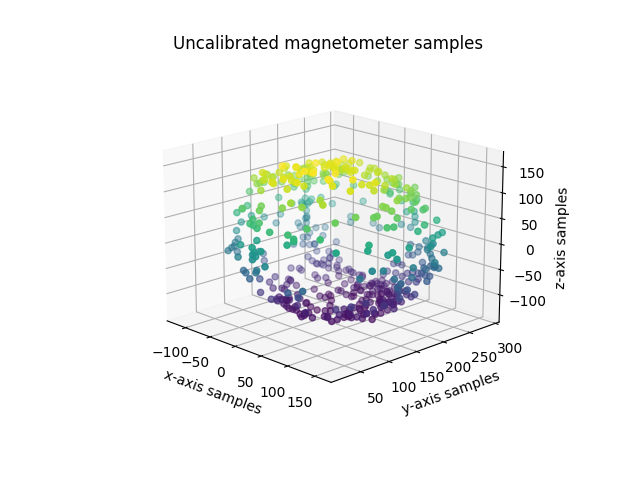
\includegraphics[width=1\linewidth]{unclibrated-mag.png}
        \caption{Uncalibrated magnetometer samples}
        \label{fig:uncalibrated}
    \end{subfigure}
    \hfill
    \begin{subfigure}[!h]{0.4\linewidth}
        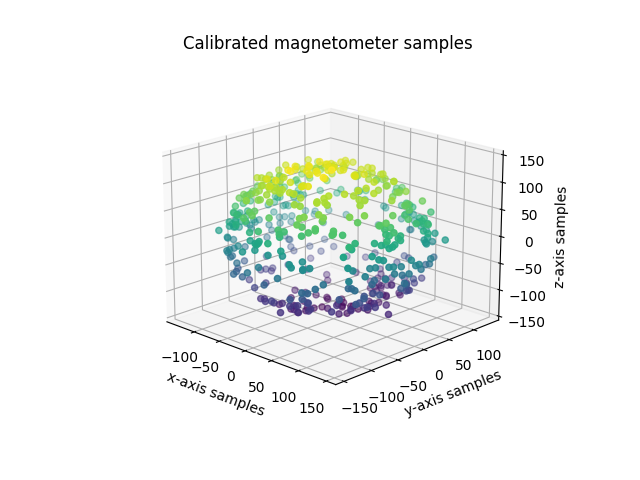
\includegraphics[width=1\linewidth]{calibrated-mag.png}
        \caption{Calibrated magnetometer samples}
        \label{fig:calibrated}
    \end{subfigure}
    \caption{Calibration process}
    \label{fig:calibration}
\end{figure}



\subsection{Digital filter}
After calibrating the digital compass and applying tilt-compensation, measurement noise was found to be present on the samples taken. A discrete second order Butterworth LPF was thus implemented to 
reduce the measurement noise. The filter parameters were determined using Scipy.signal.butter(), in Python. Different cutt-off frequencies for the filter were experimented with, the cutt-off frequency 
that produced minimal deviation on the output of the signal, as well as sufficiently low response time to a step input was chosen. 

Five hundred samples were taken with at a sample period of 70 ms, the digital compass was placed on a flat surface with a heading of $90^{\circ}$ (verified by the handheld magnetic compass). The mean
value of the samples was $89.634^{\circ}$, and variation from the mean was found to be $7.747^{\circ}$. To determine the optimal cutt-off frequency of the LPF filter, the filter was applied to the
samples, each time with a different cutt-off frequency, and the resulting deviation at the output was measured. To determine the response time of the filter to varying cutt-off frequencys, five 
hundred samples were again taken, but this time the digital compass was rotated $90^{\circ}$ during sampling to produce a step input for the filter, response times were then measured to this step input.
The reulting deviation at the output and response times for the varying cutt-off frequencies is shown in table\ref{table:filter}. The cutt-off frequency is shown in the discrete domain, therefore to 
determine the corresponding frequency in the continuous time domain simply multiply by the sampling frequency, which is 14.286 Hz.

\begin{table}[!h]
    \centering
    \caption{Response time and deviation for different LPF cutt-off frequencies}
    \label{table:filter}
    \begin{tabularx}{\columnwidth}{ | X | X | X | }
        
        \hline
        Cutt-off frequency & Response time (ms) & Variance (degrees)\\
        \hline
        0.3 &  137 & 4.0512 \\
        \hline
        0.25 &  161 & 3.4841 \\
        \hline
        0.2 &  234 & 2.9346 \\
        \hline
        0.15 &  363 & 2.3633 \\
        \hline
        0.12 &  492 & 2.1912 \\
        \hline
        0.1 &  630 & 1.7741 \\
        \hline
        0.05 &  1282 & 1.0558 \\
        \hline
    \end{tabularx}
\end{table}

A cutt-off frequency of 0.12 rad/sample was chosen as it corresponds to a response time of under 500 ms, and a sufficiently low deviation on the output. Fast response time is important in 
this specific application in order to correct the heading of the vessel quickly, should it go off course.

The transfer function of a discrete second-order Butterworth LPF is shown in Eq.\ref{eq:filter_tf}. The parameters found for a cutt-off frequency of 0.12 rad/sample are shown in 
Eq.\ref{eq:filter_b} and Eq.\ref{eq:filter_a}

\begin{equation}
    \label{eq:filter_tf}
    Y(z) = \left( \frac{b_{0} + b_{1}z^{-1} + b_{2}z^{-2}}{a_{0} + a_{1}z^{-1} + a_{2}z^{-2}} \right) \cdot X(z)
\end{equation}


\begin{equation}
    \label{eq:filter_b}
    b = (0.02785977, 0.05571953, 0.02785977) 
\end{equation}


\begin{equation}
    \label{eq:filter_a}
    a = (1. , -1.47548044, 0.58691951)
\end{equation}

The LPF filter is then implemented in software as a difference equation shown in Eq.\ref{eq:filter_code}. The filter was applied to the raw magnetometer and raw accelerometer samples (raw means 
before tilt-compensation is applied), this was done to avoid a erronous heading being returned that occurs when samples cross back and forth over $0^{\circ}$. Applying
the filter to the accelerometer samples will reduce signal noise caused by high frequency vibrations that occur during a jybe manouvre, due to the sail swapping over.


\begin{equation}
    \label{eq:filter_code}
    y[n] = \frac{b_{0}x[n] + b_{1}x[n-1] + b_{2}x[n-2] - a_{1}y[n-1] - a_{2}y[n-2]}{a_{0}}
\end{equation}


The output of the digital LPF filter designed using a cutt-off frequency of 0.12 rad/sample is shown in Fig.\ref{fig:lpf_output}, and the step response to a $90^{\circ}$ step change is shown in
Fig.\ref{fig:filter_step}.

\begin{figure}[!h]
    \centering
    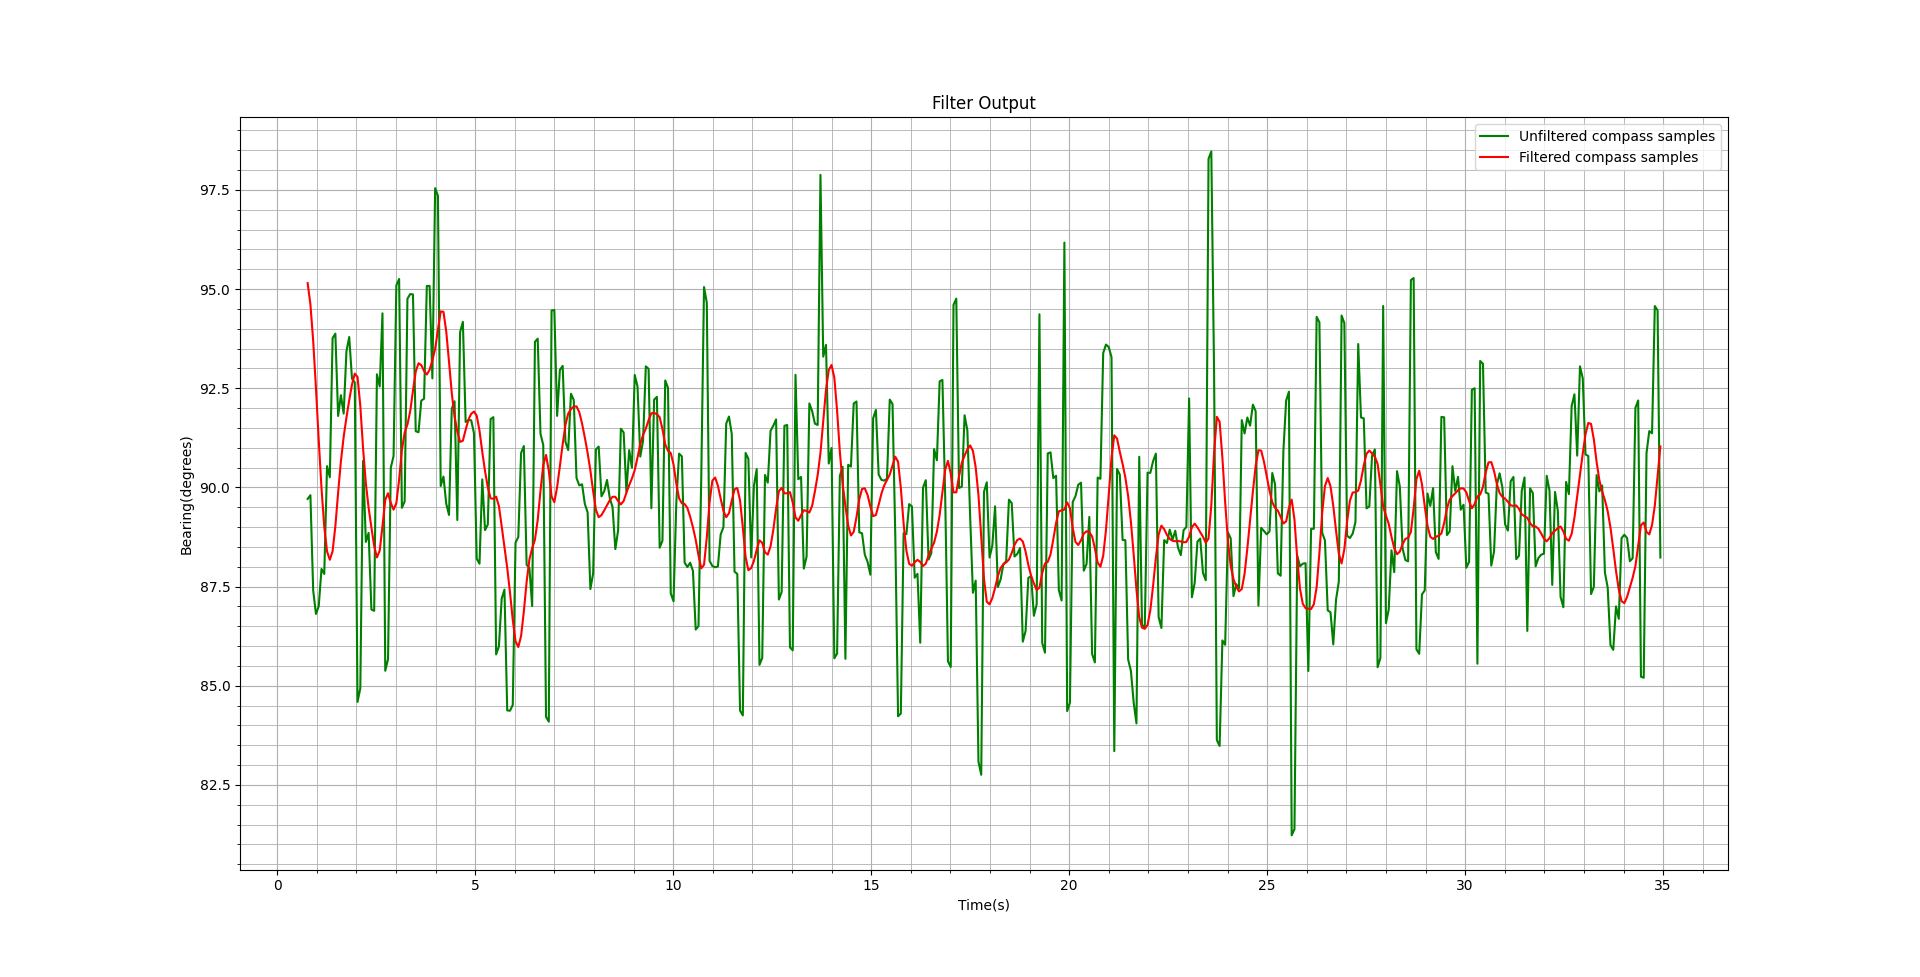
\includegraphics[width=0.98\linewidth]{Filter_output.png}
    \caption[Digital compass discrete LPF output]{Discrete LPF output}
    \label{fig:lpf_output}
\end{figure}

\begin{figure}[!h]
    \centering
    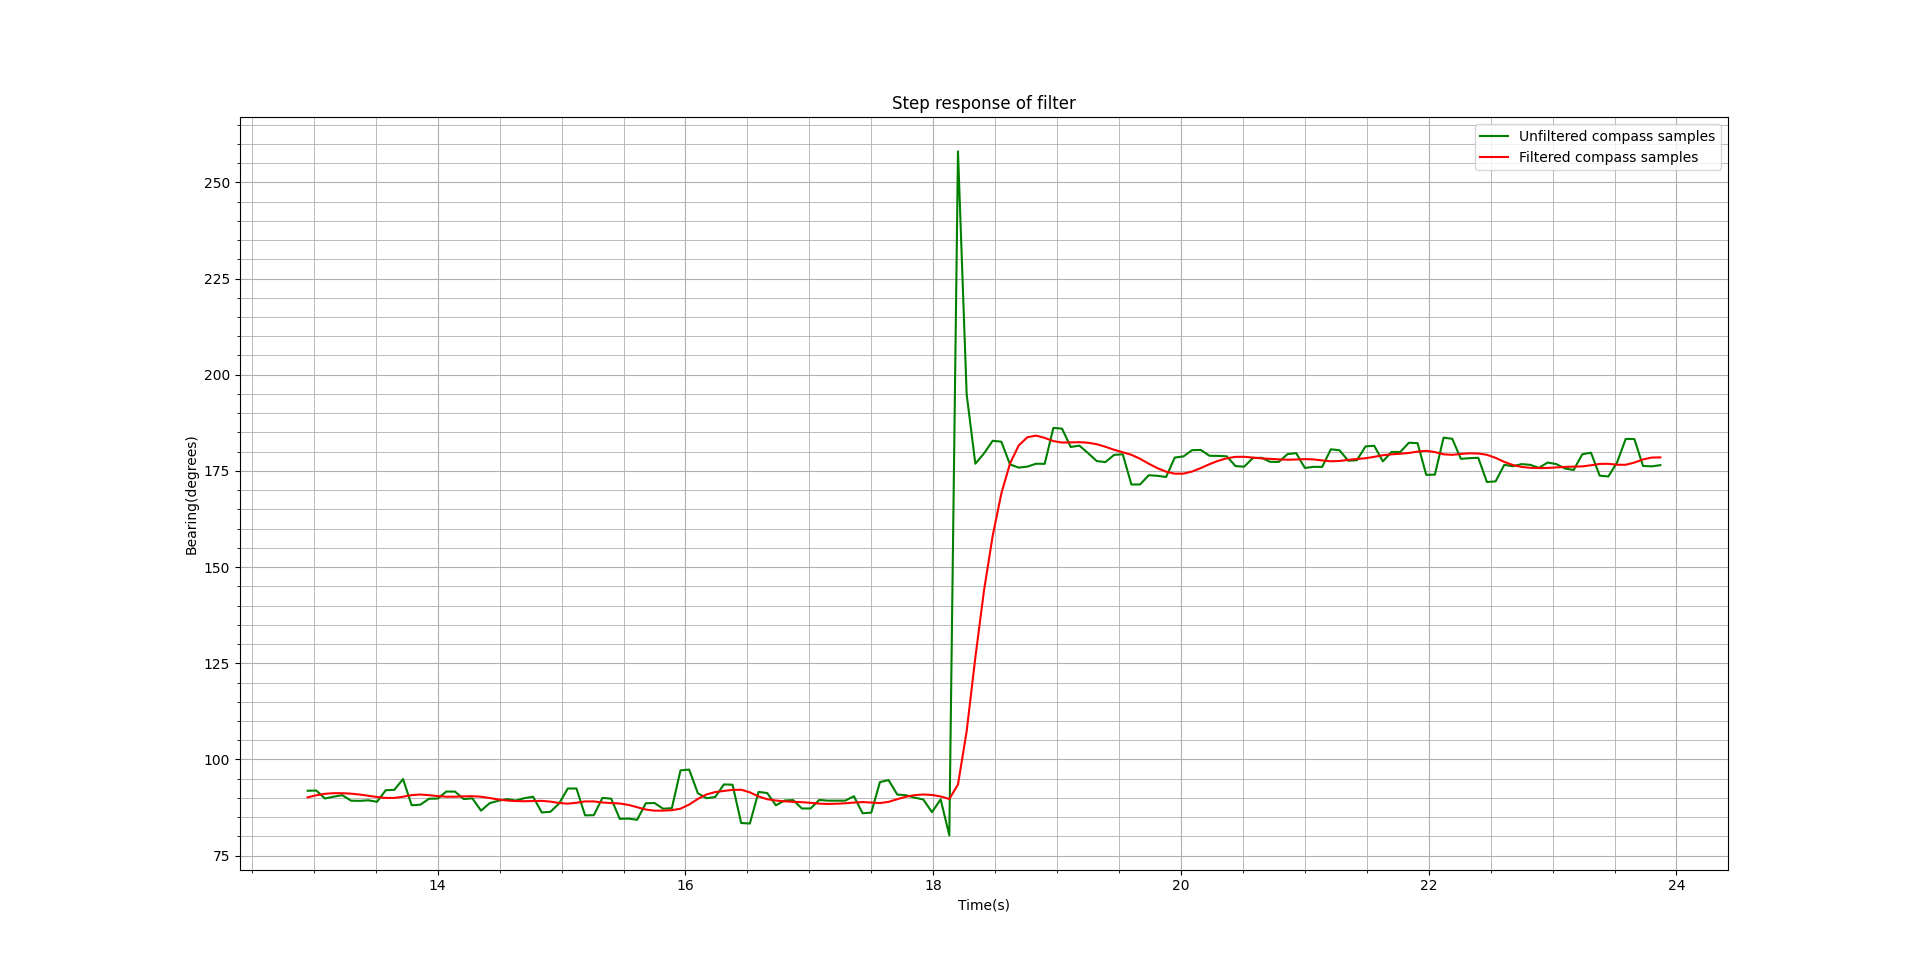
\includegraphics[width=0.98\linewidth]{Step_response.png}
    \caption[Digital compass discrete LPF step response]{Discrete LPF step response}
    \label{fig:filter_step}
\end{figure}

\section{Power System}
%Must still measure current draw of servo motors
The Adafruit feather consumes a maximum of 80 mA when operating, the MPU-9250/6500 consumes 3.7 mA, the GPS receiver consumes 100 mA and the SD card uses 30 mA when writing or reading data. The
data-sheet for the FST200-202 does not specify power consumption, the maximum current draw was however measured to be 34.2 mA. The overall current draw of the system is therefore 247,9 mA. A 
9V Duracell battery has a milli-amp hour capacity of 310 mAh at 100 mA discharge\cite{mah}. If two 9V batteries connected in series are used to power the entire system, then the battery life will 
be less than 1,25 hours. If the two 9V batteries are used to power the wind sensor only, their life will be expanded to roughly 9,064 hours. The decision was therefore made to use the two 9V batteries to power the 
wind sensor alone, and have a separate power source for the micro-controller, GPS module, digital compass and SD card. A 5000mAh 3.7V lithium polymer battery was used to power the Adafruit feather
board. The feathers 3.3V regulator was then used to power the GPS receiver, MPU-9250/6500 IMU and SD card. The Adafruit feathers datasheet specifies that the 3.3V regulator is capable of deliverin
500 mA peak (not continuous)\cite{feather}. The combined current draw of the GPS receiver, MPU-9250/6500 IMU and SD card is 133,7 mA, which is much lower than the peak specification. The decision was made
to use the power source already present in the RC sailboat to power the two servo motors. The RC sailboat was designed to operate with a 6V power source (four 1.5V
alkaline batteries in series) for the two servo motors.  

\section{PCB}
A printed circuit board was designed using Altium Designer and printed with a LPKF 62 routing machine. The PCB was designed for the Adafruit feather, the GPS receiver, the MPU-9250/6500 and the 
micro-SD card socket. The PCB has input pins for the 3.7V lithium polymer battery and the 18V power source, the wind sensor connects to the board via a screw terminal and the two servo motors
connect to the board with dedicated pins. A power plane was used to distribute ground potential to all the components. The PCB has only one side of copper plating. Component schematics and footprints
were made from scratch. Fig.\ref{fig:pcb} shows a schematic of the PCB design, the system diagram used to generate the PCB schematic can be found in appendix\ref{appen:system}.

\begin{figure}[!h]
    \centering
    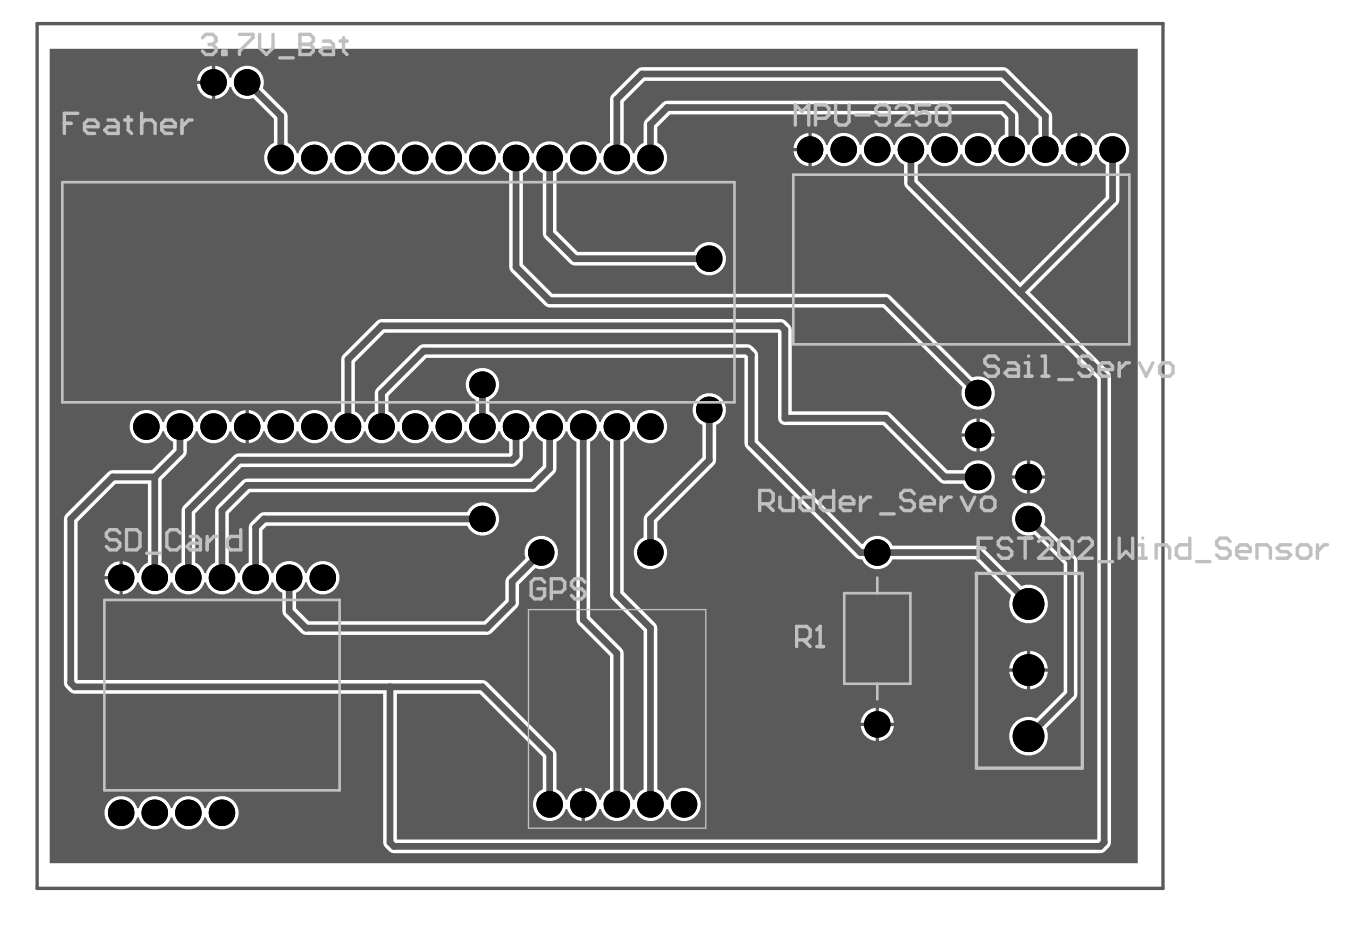
\includegraphics[width=0.8\linewidth]{system_pcb.png}
    \caption[PCB schematic]{PCB schematic}
    \label{fig:pcb}
\end{figure}



\section{Software}

\subsection{Control systems}
The control systems of the vessel consist of the rudder controller and the sail controller. Fig.\ref{fig:control-system} isllustrates the architecture of the control system. The reference signal
for the system is the heading between the current GPS-coordinates and the target GPS-coordinates, the actual heading (measured with the digital compass) is subtracted from the reference heading
to create the error signal for the rudder controller. The rudder controller then controls the rudder actuator (servo motor). 
The wind direction sensor determines apparent wind direction, this 
is then input to the sail controller, which adjusts the sail position with a control signal sent to the sail actuator.

\begin{figure}[!h]
    \centering
    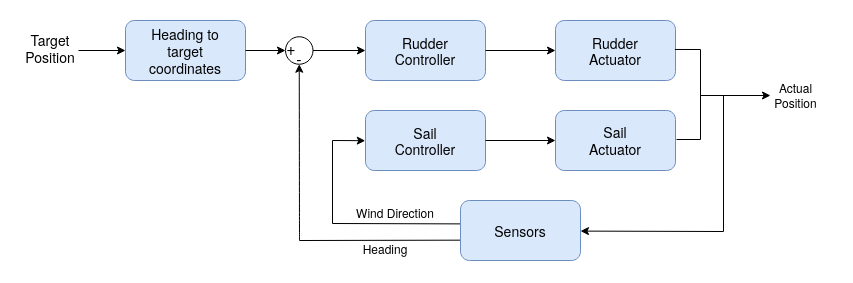
\includegraphics[width=0.98\linewidth]{control_system.png}
    \caption[Control system]{control system}
    \label{fig:control-system}
\end{figure}


\subsubsection{Sail controller}

The ADC that samples the wind direction sensors output returns a value in the range of 0 to $2^{16}$. Table \ref{table: ...} shows the minimum and maximum voltage values measured at the output of 
the sensor and the corresponding sampled ADC values expressed as a percentage. 

\begin{table}[!h]
    \centering
    \caption{Wind direction sensor output limits}
    \label{table:adc-limits}
    \begin{tabularx}{\columnwidth}{ | X | X | X | }
        
        \hline
         &Measured Voltage & ADC sampled value (\%)\\
        \hline
        Minimum & 642mV & 19.63\%  \\
        \hline
        Maximum & 3.07V & 93.1152\%  \\
        \hline
    \end{tabularx}
\end{table}

Eq.\ref{eq:sail-control-alpha} is implemented to remove the 642mV offset and convert the sampled ADC value to a value in the range $0^{\circ}$ to $360^{\circ}$. This value therefore represents the
direction of apparent wind. The cross-over point is the point where the voltage output of the sensor changes from a maximum to a minimum i.e. the voltage drops from 3.07V to 642mV. This drop does 
not occur instantaneously and because of this erronous readings can occur if samples are taken at the cross-over point. The controller was therefore designed with the wind sensor orientated such that 
the cross-over point lies in the no-sail zone, as readings taken in this area are not used anyway.


\begin{equation}
    \label{eq:sail-control-alpha}
    \alpha = \left( \frac{ADC_{sample} - ADC_{min}}{ADC_{max} - ADC_{min}} \right) \cdot 360^{\circ}
\end{equation}


When designing the sail controller the limits of the sail vessel must be taken into account i.e. the no sail zone. The sail position must be at $10^{\circ}$ when the apparent wind is $\pm 45^{\circ}$,
and sail position must be at $80^{\circ}$ when apparent wind is at $\pm 180^{\circ}$. Eq.\ref{eq:sail-control-algorithm} implements these requirements using PWM maximum and minimum values measured and recorded in table
\ref{table:pwm}. The duty cycle of the PWM signal used for the sail servo winch is stored in a 16 bit register, and is set using Eg.\ref{eq:duty_cycle}.

\begin{equation}
    \label{eq:sail-control-algorithm}
    PWM_{val} = \left( \frac{\alpha - 45^{\circ}}{180^{\circ} - 45^{\circ}} \right) \cdot \left( PWM_{max} - PWM_{min}\right) + PWM_{min}
\end{equation}

\begin{equation}
    \label{eq:duty_cycle}
    duty\_cycle = \left(\frac{PWM\_value}{1000}\right) \cdot 2^{16}
\end{equation}


\subsubsection{Rudder Controller}
%Just using proportional control for now  
The rudder controller can be designed through simulation, using the methods described in subsection \ref{sec:robotics-paper}, or by adjustment through experimentation. To design a rudder 
controller using simulation methods, the dynamics of the sail vessel need to be determined, which is not a trivial task. Eq.\ref{eq:sail_dynamics} is used to calculate and model the dynamics 
of a sail vessel, and involves calculating hydrodynamics, moment of inertia, viscous damping, lift, effort sail and centre of mass. From results in subsection \ref{sec:robotics-paper}, 
it is clear that the controller parameters determined through simulation were not optimal and therefore design rudder controller for this project is done by adjustment.

The rudder controller used is a proportional controller. The control law for this controller is shown in Eq.\ref{eq:control-law}, where $k_{p}$ is the proportional gain and $E_{r}$ is the 
error signal. The error signal is determined using Eq.\ref{eq:error-sig}, where $\psi_{r}$ is the reference bearing and $\psi_{a}$ is the actual bearing of the vessel. 

\begin{equation}
    \label{eq:control-law}
    U[k] = k_{p}E_{r}
\end{equation}

\begin{equation}
    \label{eq:error-sig}
    E_{r} = \psi_{r} - \psi_{a}
\end{equation}

After calculating the error signal a check is done in software: if the error signal is greater than $180^{\circ}$ then subtract $360^{\circ}$, and if the error signal is smaller than $180^{\circ}$
then add $360^{\circ}$, else do nothing. This check is done to ensure that the vessel turns in the direction associated with the smallest angle of correction. For example: if the angle of correction
in the clockwise direction is $100^{\circ}$ and $60^{\circ}$ in the anti-clockwise direction, the boat will turn anti-clockwise.

Eq.\ref{eq:pwm-sig-rudder} is used to determine the duty cycle - Eq.\ref{eq:duty_cycle} - of the PWM signal that controls the rudder servo. The maximum and minimum PWM values measured in table \ref{table:pwm}
are used here.

\begin{equation}
    \label{eq:pwm-sig-rudder}
    PWM_{val} = \left( \frac{U[k]}{60^{\circ}} \right) \cdot (PWM_{max} - PWM_{min}) + \left( \frac{PWM_{max} + PWM_{min}}{2} \right)
\end{equation}

\subsection{Navigational calculations}
\subsubsection{Distance}
To calculate distance over the surface of a sphere two options were considered: The Haversine formulae and the equirectangular approximation. The Haversine formulae is more accurate but can be 
computationally expensive, the equirectangular approximation is less accurate but more efficient. The Haversine formulae was chosen as the accuracy is required. The Haversine formulae is shown 
in Eq.\ref{eq:haversine1} and Eq.\ref{eq:haversine2}, where
the current coordinates are $(lat_1, long_1)$ and the target coordinates are $(lat_2, long_2)$, R is the radius of the earth in km. Coordinates are in decimal degrees.

\begin{equation}
    \label{eq:haversine1}
    a = sin^{2}\left( \frac{lat_{2} - lat_{1}}{2}\right) + cos(lat_{1})\cdot cos(lat_{2})\cdot sin^2\left(\frac{long_{2} - long_{1}}{2}\right)
\end{equation}

\begin{equation}
    \label{eq:haversine2}
    d = R\cdot \left(2\arctan\left(\frac{\sqrt{a}}{\sqrt{1-a}}\right)\right)
\end{equation}


Eq.\ref{eq:haversine1} returns values in the order of $e-17$ for a 
distance on 1m. In Python floats are single precision numbers with a maximum value of $\pm3.4e38$ and minimum value of $\pm1.7e-38$, therefore the haversine function can be used to determine 
small distances on the micro-controller. 

\subsubsection{Heading}
To calculate reference heading Eq.\ref{eq:ref-heading} is used.

\begin{equation}
    \label{eq:ref-heading}
    \psi_{r} = \arctan\left( \frac{sin(long_2 - long_1)cos(lat_2)}{cos(lat_1)sin(lat_2) - sin(lat_1)cos(lat_2)cos(long_2 - long_1)}\right)
\end{equation}


\subsection{Program flow}


